%% Goal clean up this section, make it concise, and finish it!

\chapter{Cryptography}
%Quick overview of cryptography

\section{Algorithm selection overview}
%Which encrypting plan will I use?

\subsection{Symmetric key encryption}
\paragraph{Selecting an algorithm, among so many, was pretty straightforward given my use case. Firstly, there are two fundamental paths for selecting an encryption algorithm. The selection between \emph{asymmetric} and \emph{symmetric} key encryption is the initial decision.}

\begin{enumerate}
\item Asymmetric-key cryptography: A public and private key are created by both people wanting to exchange encrypted emails. This is the most secure and most commonly implemented encryption available, popularly known as "public-key encryption." Examples encryption key algorithms used include RSA and Diffe-Hellman-Merkle. \cite[Website]{Shirey}
\item There are challenges though:
\begin{enumerate}
\item Both parties need to create their own keys
\item Keys need to be exchanged, i.e. a person has to be acute enough to search for the other person's public key -- assuming one even exists
\item Additional client software is also often required
\end{enumerate}
\item Symmetric-key encryption: Use the same key for both encryption and decryption \cite[p. 155]{DelfsKnebl}
\begin{enumerate}
\item The primary drawback is both parties need to exchange that single key, often times in the form of a password.
\end{enumerate}
\end{enumerate}

\paragraph{The goal of this project is \emph{ease of use} (at the cost of security), so our choice is clear: symmetric-key encryption.}

\subsection{Block vs. Stream cipher encryption}
\paragraph{Next, we need to decide between a block cipher or a stream cipher. As Bruce Schneier defines the two in his book "Applied Cryptography: Protocols, Algorithms in C" as:}

\begin{quote}
"There are two basic types of symmetric algorithms: block ciphers and stream ciphers. Block ciphers
operate on blocks of plaintext and ciphertext—usually of 64 bits but sometimes longer. Stream
ciphers operate on streams of plaintext and ciphertext one bit or byte (sometimes even one 32-bit
word) at a time. With a block cipher, the same plaintext block will always encrypt to the same
ciphertext block, using the same key. With a stream cipher, the same plaintext bit or byte will
encrypt to a different bit or byte every time it is encrypted." \cite[p. 12]{Schneier}
\end{quote}
\paragraph{The advantages of a stream ciphers:}

\begin{itemize}
\item bit (or byte) at a time encryption
\item speed of encryption/decryption
\end{itemize}

\paragraph{are more appropriate for hardware implementations.}

\paragraph{According to Bruce Schneier, block ciphers are more suitable for software implementation as they are easier to implement, avoid time-consuming bit manipulations, and operate on computer sized blocks.}\cite[p. 172]{Schneier}

\subsection{Block cipher selection}
\paragraph{There are many block ciphers to choose from, these are just some of the most popular:}\cite{Nirula}
\begin{enumerate}
\item Digital Encryption Standard (DES): DES is a symmetric key block cipher that uses 64-bit blocks, but it has been found vulnerable to powerful attacks. This is the reason the use of DES is on a decline. 
\item Triple DES: This symmetric key cipher uses three keys to perform encryption-decryption-encryption. It is more secure than the original DES cipher but as compared to other modern algorithms, triple DES is quite slow and inefficient. 
\item Advanced Encryption Standard (AES): AES has superseded the DES algorithm and has been adopted by the U.S. government. It is a symmetric key cipher and uses blocks in multiple of 32 bits with the minimum length fixed at 128 bits and the maximum at 256 bits. The algorithm used for AES, was originally named Rijndael.\footnote{The winners of the AES competition were two Belgians: Vincent Rijmen, Joan Daemen, thus the algorithm's name: "\textbf{Rij}n\textbf{dae}l"}
\item Blowfish: Blowfish is a symmetric key block cipher with a block size of 64 and a key length varying from 32 bits to 448 bits. It is unpatented, and the algorithm is available in the public domain. 
\item Twofish: Twofish is also a symmetric key block cipher with a block size of 128 bits and key sizes up to 256 bits. It is slower than AES for 128 bits, but faster for 256 bits. It is also unpatented and the algorithm is freely available in the public domain.
\end{enumerate}

\paragraph{After an overall account of the available block enciphers, the author decided there is really only one choice: the Advanced Encryption Standard (AES) as it's the industry standard.}

\section{Advanced Encryption Standard (AES)}

\paragraph{For reasons that will soon become apparent, AES has been the industry standard for the past 20 years, even used as a secure standard by the U.S. government.} \cite [p. 107]{Aumasson}

%Describe the mathematics involved in the Algorithm.

\subsection{Mathematics: Overview}
\paragraph{Since a full background is beyond the scope of this project (it could entail it's own thesis), the author will gloss over it quickly.}
%Start with Field Theory - Galois

\paragraph{The foundation of AES is grounded in Abstract mathematics, more specifically, \emph{set theory}. Within set theory exists the study of groups. A group is a set of elements upon which an operation (and its inverse) can be executed.}\cite[p. 92]{PaarPelzl} 

\paragraph{In short,}

\begin{enumerate}
\item addition
\item subtraction
\item multiplication
\item division
\end{enumerate}

\paragraph{are operations that can be applied to a group of elements.}

\paragraph{A field is an extension of a group, in that all four basic arithmetic operations are included in a single structure.}\cite[p. 92]{PaarPelzl} 

\paragraph{However, as cryptographers, we are not yet satisfied. We need a working set that is finite, or as they are commonly known \emph{Galois fields}, or \emph{endliche Körpe}. In short, the beauty of the Galois fields is that regardless of the four principle operations performed on them, the result will remain \emph{within} the set of elements. This is profound, necessary and brilliant for cryptographic usage. But, how does this work?} \cite [Website]{PaarYoutube}

\paragraph{Essentially, the above operations are carried out with the aid of the \emph{modulo operator}, and it ensures our result remains in the set. But, what set?}

\paragraph{The Galois field principles are focused on one particular sub-field, namely the field defined by:}

$GF(2^8)$

\paragraph{This conveniently translates to 256 elements, which fits perfectly within a computer byte.}

\paragraph{The last thing we will want to have in mind as we proceed is polynomial division. It's not any different than grammar school algebra, but is carried out with one of a very special type of polynomial, known as a \emph{irreducible polynomial}. An irreducible polynomial is similar to a prime number, only that it is a polynomial. In other words, it cannot be factored into smaller components. The AES algorithm uses the following polynomial: $x^8 + x^4 + x^3 + x + 1$}\cite[p.21]{DelfsKnebl}

\subsection{The AES algorithm}

\paragraph{With the mathemathical theories out of the way, we can look at how all the theory get implemented into our computers. Here is a simplifed overview: (See: \ref{fig: AESovereview}).}


\begin{figure}[H]
\centering
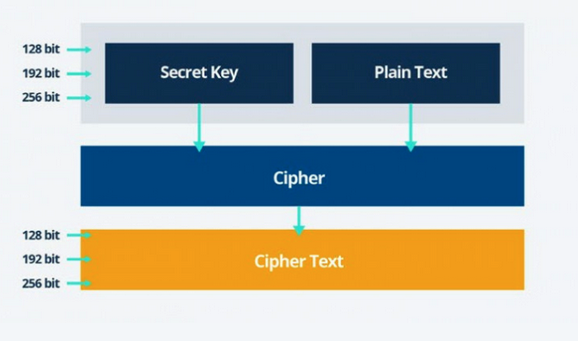
\includegraphics[width=0.9\textwidth]{simplifiedOverviewAES.png}
\caption{\label{fig: AESovereview} Simplified AES Overview}\cite[Webpage]{Crawford}
\end{figure}


\paragraph{The first step in the AES algorithm is the creation of a 4-by-4 array of bytes called the state, that is modified in a series of rounds. The state is initially set equal to the input of the cipher (notice: a 128 bit minimum is exactly 16 bytes, perfect for execution on a computer). Then, the following four operations are applied.}\cite[p. 186]{Katz}

%the following images need to be cited!
\subsection{Step one: "AddRound" key}
\paragraph{In every round of the AES, a 128-bit sub-key is derived from the master key, and it is interpreted as a 4-by-4 array of bytes. The state array is updated by XORing it with the sub-key (See: \ref{fig: AddRoundKey}).}\cite[p. 186]{Katz}

\begin{figure}[H]
\centering
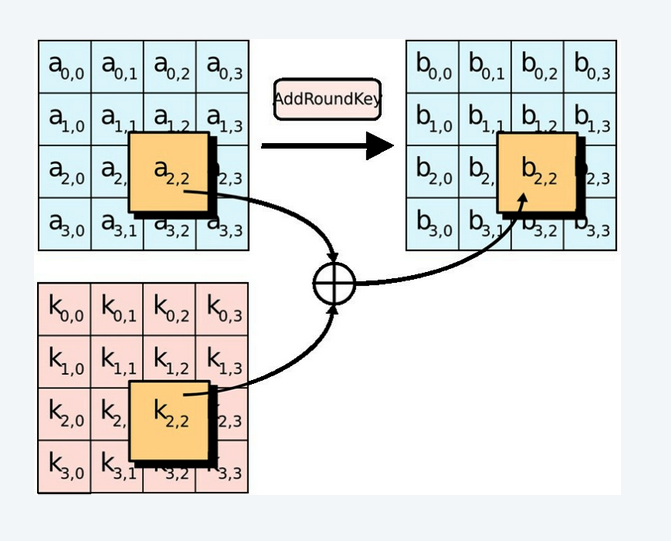
\includegraphics[width=0.8\textwidth]{AddRoundKey.png}
\caption{\label{fig: AddRoundKey} AddRound Key Round}\cite[Webpage]{Crawford}
\end{figure}


%Byte substitution - bit shifting?
\subsection{Step two: "SubBytes" or byte substitution}
\paragraph{In this step, each byte of the state array is replaced by another byte according to a single fixed table S. This substitution table (or S-box) is a bijection over $\{0,1\}^8$. There is only one S-box that is substituting all the bytes in the state array, every round (See: \ref{fig: SubBytes}).}\cite[p. 186]{Katz}

\begin{figure}[H]
\centering
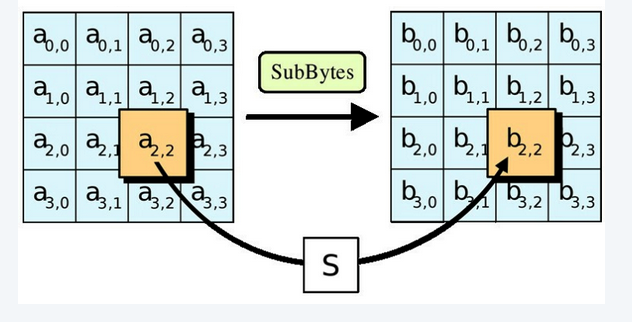
\includegraphics[width=0.8\textwidth]{SubBytes.png}
\caption{\label{fig: SubBytes} SubBytes Round}\cite[Webpage]{Crawford}
\end{figure}


%Row Shifting
\subsection{Step three: "ShiftRows" or the rows are shifted}
\paragraph{In this step, the bytes in each row of the state array are cyclically shifted to the left as follows: the first row of the array is untouched, and the second row is shifted one place to the left, the third row is shifted two places to the left, and the fourth row is shifted three places to the left (See: \ref{fig: ShiftRows}).}\cite[p. 186]{Katz}

\begin{figure}[H]
\centering
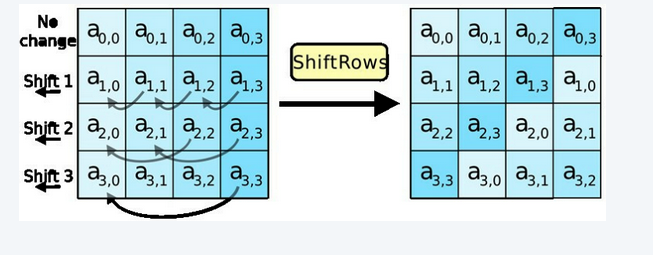
\includegraphics[width=0.8\textwidth]{ShiftRows.png}
\caption{\label{fig: ShiftRows} ShiftRows Round}\cite[Webpage]{Crawford}
\end{figure}

%Column mixing??
\subsection{Step four: "MixColumns" or the columns are mixed}
\paragraph{In this step, an invertible linear transformation is applied to each column. One can think of this as a matrix multiplication (See: \ref{fig: MixColumns}).}\cite[p. 186]{Katz}

\begin{figure}[H]
\centering
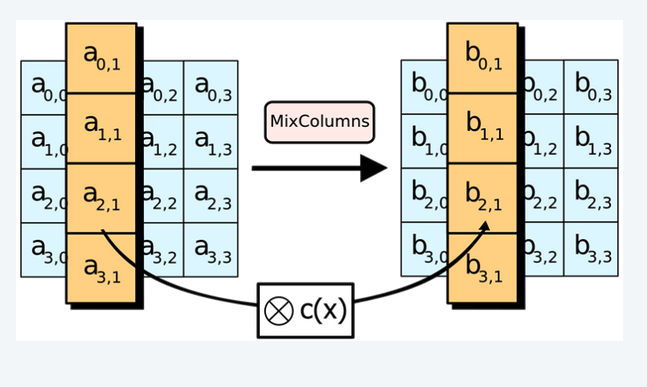
\includegraphics[width=0.8\textwidth]{MixColumns.png}
\caption{\label{fig: MixColumns} MixColumns Round}\cite[Webpage]{Crawford}
\end{figure}

%Algorithm (all the above) is repeated 9-13 times, depending on bit level of encryption.
\subsection{The process is repeated x number of times}
\paragraph{The AES algorithm supports bit sizes of 128 (minimum requirement), 192, and 256. Depending on the bit size specified, the algorithm will be repeated either 10, 12, or 14 times.}



% Goal to achieve Diffusion and Confusion.
\subsection{AES algorithm summary}
\paragraph{The goal of the algorithm is to insert confusion and diffusion into the field, over and over. And, the algorithm is just reversed to retrieve the plain text. The algorithm was fast in 2001, when it was introduced, but now, 20 years later, it is built into all modern CPUs, so it's blazingly fast.}

\paragraph{Although the algorithm is derived from a combination of complex mathematical theories, its algorithmic implementation into hardware is the perfect intersection between mathematics and computer science. Any computer scientist can quickly assess from the images above, that the XORing, bit shifting, table lookups, and bit permutations are exactly the kind of operations that are executed super fast on computers.}\cite[p. 178]{Dooley}


